%! suppress = MissingLabel
%! suppress = EscapeAmpersand

Искусство программирования во многом состоит в умении управлять сложностью, и в рамках данного курса основным инструментом для этого мы будем рассматривать построение языков и интерпретаторов.

\subsection{Интерпретаторы как основа основ}

Мы начнём с обзора роли интерпретаторов в программировании.

\subsubsection{Башня интерпретаторов} \label{subsec:interpreters-tower}

Самым базовым интерпретатором является процессор, он воплощён физически в железе.
Ему на вход подаётся программа на некотором языке, например, x86, он зачитывает команды и превращает их в действия над памятью.
Однако, человеку сложно программировать на этом языке, нужен новый язык, инкапсулирующий часть сложности и скрывающий лишние детали.

Чтобы получить новый язык, мы строим программный интерпретатор.
\vocab{Программный интерпретатор} $U_M^N$ --- это программа на языке $M$\footnote{Под языком мы тут понимаем множество программ на этом языке, иначе говоря, множество деревьев определённого вида.}, получающая на вход программу на языке $N$ и вход для неё --- данные из $D$, и возвращающая результат выполнения этой программы на этих данных: \[U_M^N : N\times D\to D\]

Язык реализации интерпретатора $M$ мы будем называть \vocab{мета-языком}, а $L$ --- \vocab{определяемым}.
Про интерпретатор можно интуитивно думать следующим образом: это понятное мета-языку объяснение того, что значат конструкции определяемого языка.
Иными словами, какие инструкции мета-языка нужно исполнить, чтобы получить нужную семантику инструкций определяемого языка.

Например, у нас есть программа $p_N$ и данные для неё $d_{in}$, результат исполнения этой программы $d_{out}$ можно получить как \[d_{out} = U_M^N\left( \underbrace{\langle p_N, d_{in} \rangle}_{\in N\times D} \right)\]

Но интерпретатор это тоже программа.
Как её запустить?
Возьмём наш базовый интерпретатор $U^{x86}$, у него нет языка реализации, так как он реализован в железе, а не программно.
Возьмём интерпретатор языка ассемблера, реализованный в кодах x86, $U_{x86}^{Asm}$, программу на ассемблере $p_{Asm}$ и вход для неё $d_{in}$.
Вспомним, что программа --- это тоже данные, просто в некотором специальном формате.
Тогда результат применения $p_{Asm}$ на данных мы получим следующим образом:
\[
    d_{out} = U^{x86}\left(\left<\underbrace{U_{x86}^{Asm}}_{\in Asm}, \underbrace{\overbrace{\langle p_{Asm}}^{\in Asm}, \overbrace{d_{in} \rangle}^{\in D}}_{\in D} \right>\right)
\]

Но язык ассемблера, тоже не очень приятен для программирования.
Однако, на нем можно уже написать интерпретатор языка посложнее.
И так далее.
Получаем \point{башню интерпретаторов}, на вершине находится язык, на котором мы хотим уже решать непосредственно нашу задачу:
\[
    d_{out} =
    U^{x86}\left(\left<
                     U_{x86}^{Asm}, \left<
                                        U^C_{Asm}, \left<
                                                       U^{Has}_C, \left< p_{Has}, d_{in}
                \right>\right>\right>\right>\right)
\]

На практике часто язык задают через трансляцию (компиляцию) в другой.
Однако, интерпретаторы, как правило, сильно проще, а так же существует универсальный теоретический способ построения компилятора по интерпретатору\footnote{\url{https://en.wikipedia.org/wiki/Partial_evaluation}}, поэтому мы сосредоточимся на интерпретаторах.

\subsubsection{Интерпретаторы повсюду} \label{subsec:interpreters-everywhere}

Хорошо, мы пришли к языку нашего сердца (Хаскеллу), почему же мы продолжаем говорить об интерпретаторах?
Потому что для решения конкретных бизнес-задач прикладные языки всё ещё слишком церемониальны~--- программисту приходится думать о большом количестве вещей, нерелевантных его предметной области и решаемой задаче.
Сложность~--- главный враг программиста, потому что ресурсы человеческого мозга несопоставимы со сложностью реальности, которую приходится описываться в программах.
Таким образом, в работе постоянно приходится описывать новые языки, наиболее подходящие для решения конкретных прикладных задач.
А новые языки мы задаём с помощью интерпретаторов.

Как выглядит классический рекурсивный интерпретатор?
Он получает программу в виде некоторого дерева и рекурсивно обходит его, считая результаты поддеревьев.
Когда он посещает вершину дерева, он определяет её тип и понимает, какие действия нужно исполнить.
То есть тип вершины диспатчит, навигирует, исполнение интерпретатора на нужный код.
Так, интерпретатор простой языка выражений имеет следующий вид:
\begin{minted}{haskell}
    eval :: Expr -> Int
    eval prog = case prog of
      Const x -> x
      Plus l r -> eval l + eval r
\end{minted}

Видно, что это похоже, например, на работу утилиты командной строки~--- разбираем аргументы, определяем, что и как нужно сделать, делаем.
Как ни странно, философия Unix, в частности, заключается в построении маленьких языков (утилит с текстовым API), решающих хорошо одну задачу~\cite{bentley1986little}.
Ещё это похоже на обработку запроса web-сервером~--- определяем роут на которую пришел запрос, выполняем соответствующее действие.
То есть не так редко мы в реальной жизни пишем интерпретаторы.
Мы просто не видим, что то, что мы пишем --- это на самом деле интерпретатор некоторого языка.
В общем случае, свёртку структуры данных уже можно рассматривать как интерпретацию~\cite{gibbons2014folding}.

Более того, как мы убедимся в дальнейшем~\ref{subsec:tagless-final}, написание любой функции~--- это уже задание нового языка.
Вот был язык, в котором нельзя было добавить пользователя в приложение.
Написали функцию \texttt{registerUser}~--- появилась новая команда в языке~--- добавить пользователя.
Также, мы формально покажем, то такой способ эквивалентен добавлению новой ноды в синтаксическое дерево языка.
Использование функций является примером встраивания языка, когда мы вместо того, чтобы делать новый отдельный язык, его реализуем как библиотеку для уже существующего языка~\cite{gibbons2013functional}.

Как мы убедимся в течение курса, многие задачи можно рассматривать как придумывание языка и реализацию интерпретатора.
Значит, если мы научимся хорошо писать интерпретаторы, мы научимся делать сразу кучу всего!
И основные наши усилия будут направлены на изучение средств построения интерпретаторов встроенных языков.

Во время повествования мы часто пользуемся приёмом Hutton's Razor, который подразумевает рассмотрение до смешного маленького языка для изучения сложных концепций.
Утверждается, что для изучения большинства вопросов можно сконструировать такой язык, делающий всё важное максимально наглядным.

\subsubsection{Интерпретаторы и семантика языков программирования} \label{subsec:semantics}

Семантика языков программирования\footnote{\url{https://en.wikipedia.org/wiki/Semantics_(computer_science)}\label{note:sema-wiki}}~--- это наука, изучающая свойства языков и смысл программ, его свойства и способы описания.
Отличным введением может послужить серия книг Software Foundations\footnote{\url{https://coq.vercel.app/ext/sf/}}~\cite{pierce2010software}.
Существует много различных стилей описания семантики программ, для нас важнейшим будет денотационная семантика.

\vocab{Денотационная семантика}\footnote{\url{https://en.wikipedia.org/wiki/Denotational_semantics}}\footnote{\url{https://en.wikibooks.org/wiki/Haskell/Denotational_semantics}}\footnote{\href{https://youtu.be/pQyH0p-XJzE?si=TUEzrpHhJZfO7dTF}{(youtube) The Lost Art of Denotational Semantics --- Eric Meyer.}} описывает смысл программ путём сопоставления им объектов некоторого множества, \vocab{семантического домена}.
Иначе говоря, денотационная семантика языка $L$ --- это тотальная функция из программы на этом языке в элемент домена $D$:
\[
    \sembr{\bullet} : L \mapsto D
\]

Домен выбирается исходя из языка и информации, которую хочется извлекать из программ.
Например, чтобы узнать размер программы (тут, выражения со сложением), в качестве домена можно взять натуральные числа:
\[
    \begin{array}{lcl}
        \sembr{n}     & = & 1                            \\
        \sembr{l + r} & = & \max{(\sembr{l}, \sembr{r})}
    \end{array}
\]
Если нас интересует конечный результат, можно посчитать его:
\[
    \begin{array}{lcl}
        \sembr{n}     & = & n                     \\
        \sembr{l + r} & = & \sembr{l} + \sembr{r}
    \end{array}
\]
Если у программы есть вход, доменом будет функция $\mathbb{N}\to\mathbb{N}$:
\[
    \begin{array}{lcl}
        \sembr{n}(m)     & = & n                           \\
        \sembr{l + r}(m) & = & \sembr{l}(m) + \sembr{r}(m) \\
        \sembr{input}(m) & = & m
    \end{array}
\]

Таким образом, программа является лишь синтаксической записью для некоторого элемента семантического домена.
Вариантов доменов много, это могут быть даже игры\footnote{\url{https://en.wikipedia.org/wiki/Game_semantics}}. % todo domain theory

\begin{task}
    В какой домен разумно проинтерпретировать программы на языке с целочисленными мутабельными переменными?
    А на недетерминированном языке?
\end{task}

Легко заметить, что денотационная семантика языка --- это просто интерпретатор, только написанный на языке математики.
Такие интерпретаторы ставят в основу башни интерпретаторов, когда цель исследовать свойства языков и программ, а не исполнять их.

Также, можем реализовывать интерпретатор на каком-нибудь реальном языке и он тоже будет задавать семантику определяемого языка.
Однако формальность такого определения будет зависеть от формальности описания семантики мета-языка.
Такие интерпретаторы называют ``\vocab{определяющими}'', они задают семантику языка, как правило, жертвуя эффективностью ради наглядности.
Взаимоотношения определяемого языка и мета-языка изучаются в классических статьях~\cite{reynolds1972definitional,reynolds1998definitional}\footnote{Активно используемое автором понятие продолжения будет рассмотрено далее в этом курсе (раздел \ref{sec:continuations}).}.

Мы будем использовать определяющие интерпретаторы для задания семантики новых языков и в качестве мета-языка будем использовать Haskell.
А в качестве доменов будем брать типы Haskell.
И интерпретировать программу не в множество функций между натуральными числами, а, скажем, в тип \mintinline{haskell}|Nat -> Nat| в языке Haskell\footnote{\url{https://okmij.org/ftp/Denotational.html}}. % todo review haskell denotational semantics
Так, денотационная семантика языка сумм с входом будет записываться следующим образом:
\begin{minted}{haskell}
    eval :: Prog -> (Nat -> Nat)
    eval = \case
      Val n -> \_ -> n
      Plus l r -> \m -> eval l m + eval r m
      Input -> \m -> m
\end{minted}

Семантика называется \vocab{композиционной (compositional)}, если смысл конструкций зависит только от смысла подконструкций.
Иначе говоря, если денотационная семантика представляет собой свёртку программы (рис.\ \ref{fig:eval-prog}) и может быть записана в терминах катаморфизма~\ref{subsubsec:recursion-schemas}.

\begin{figure}[h]
    \centering
    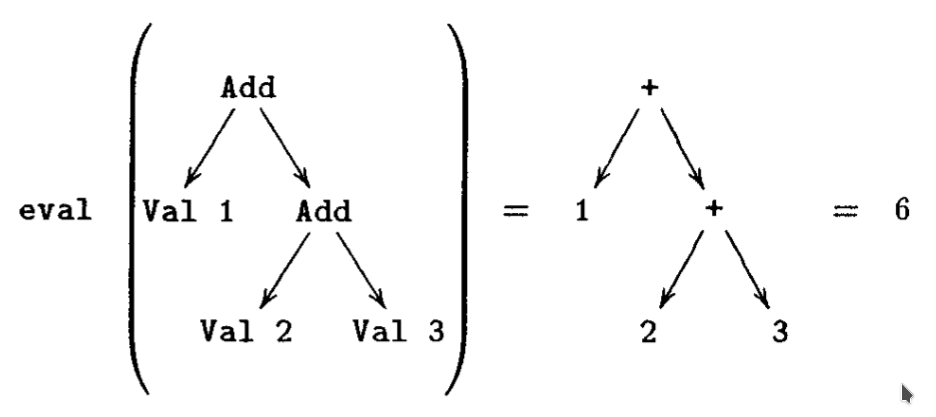
\includegraphics[width=0.6\textwidth]{figs/eval-prog}
    \caption{Денотационная семантика определяет смысл синтаксических конструкций через операции над доменом~\cite{hutton1998fold}.}
    \label{fig:eval-prog}
\end{figure}

Другим популярным стилем описания семантики является \vocab{операционная семантика}, которая представляет смысл программы в виде последовательности шагов вычислений.
Это может быть как последовательное переписывание самого выражения, так и переписывание состояния некоторой абстрактной машины.
Операционная семантика, в свою очередь, задаётся как развёртка (или анаморфизм~\ref{subsubsec:recursion-schemas}) последовательности шагов вычисления из программы.
Тут отчётливо видна некоторая двойственность между денотационной и операционной семантиками~\cite{hutton1998fold}.

\subsubsection{Встроенные доменно-специфичные языки (eDSL)} \label{subsubsec:edsl}

Под \vocab{доменно-специфичными языками (domain specific languages, DSL)}\footnote{\url{https://en.wikipedia.org/wiki/Domain-specific_language}} часто понимают специализированные языки для конкретных предметных областей, например, запросов к БД или форматирования документов.
Как правило, такие языки не являются полными по Тьюрингу.

В этом курсе, однако, мы будем считать доменно-специфичным языком любую доменно-специфичную специализацию языка общего назначения\footnote{\url{https://en.wikipedia.org/wiki/Language-oriented_programming}, на русскоязычную страницу тоже следует заглянуть.}.
Это следует из того соображения, что код должен читаться как грамотная проза с уместным словоупотреблением, предоставляющая читателю только необходимое количество подробностей, скрывая несущественное за умолчаниями и терминологией.

\vocab{Самостоятельные доменно-специфичные языки (standalone domain specific languages)} --- языки, имеющие свой собственный конкретный синтаксис, а так же инструменты программирования (IDE, исполняющая среда\ldots).
Примеры: SQL, AWK, Antlr\ldots\footnote{Есть отличная прикладная книга~\cite{nystrom2021crafting}, рассказывающая о построении интерпретаторов и простых виртуальных машин.
В то же время она покрывает сознание полноценного языка во всех его аспектах, от синтаксического анализа до управления памятью.}

\vocab{Встроенные доменно-специфичные языки (embedded domain specific languages, eDSL)} --- языки, пользующиеся поддержкой инфраструктуры других языков.
Обычно реализуются как библиотеки для программ на уже существующем языке общего назначения.
Не имеют полностью собственного конкретного синтаксиса.
Примеры: ORM, функции обработки строк, библиотека парсер-комбинаторов\ldots

\vocab{Deep eDSL} --- термы на таком языке строят дерево абстрактного синтаксиса для дальнейшей интерпретации:
\begin{minted}{haskell}
    f :: Int -> Int
    f = eval $ Const 1 `Plus` Input
\end{minted}

Интерпретаторы, которые принимают деревья на вход и интерпретируют их в семантический домен, называют \vocab{инициальными}\footnote{Тип синтаксиса заданный с помощью \mintinline{haskell}{data} является инициальным объектом категории интерпретаций.}, мы их также будем называть ``классическими''.
С них мы и будем начинать.
Классические интерпретаторы полезны, например, как для реализации ``последнего языка''~--- интерфейса программы во внешний мир, и как фундамент для наших дальнейших построений.

%Например, можно построить встроенный язык для работы с изменяемым состоянием.
%Теперь можем писать императивно в Haskell без единой монады!
%\begin{minted}{haskell}
%    fac :: Int -> Int
%    fac = eval $
%
%\end{minted}

Однако, можно заметить, что промежуточное дерево, которое получается, нас, как правило, не интересует.
Нам важно только получить элемент домена, которым мы уже умеем пользоваться непосредственно.
\vocab{Shallow eDSL} минуют стадию построения дерева и сразу строят значение в семантическом домене.
Такие интерпретаторы мы будем называть \vocab{финальными}\footnote{Такой способ задания интерпретаторов называют финальным по историческим причинам. Казалось, что соответствующие программы соответствуют терминальному (финальному) объекту категории интерпретаций. Однако, как оказалось, с категорной точки зрения, это тоже инициальный объект.}.
\begin{minted}{haskell}
    cnst :: Int -> (Int -> Int)
    cnst x _ = x

    input :: Int -> Int
    input env = env

    plus :: (Int -> Int) -> (Int -> Int) -> (Int -> Int)
    plus l r env = l env + r env

    f :: Int -> Int
    f = cnst 1 `plus` input
\end{minted}

Интерпретаторы часто называют \vocab{наблюдателями (observers)}, которые анализируют термы и дают им некоторый смысл~\cite{gibbons2013functional}.
Можно заметить, что для deep eDSL можно написать сколь угодно много различных наблюдателей.
Однако в случае shallow embedding наблюдатели всегда \texttt{id}.
Мы будем обсуждать возможные решения этой проблемы далее в разделе~\ref{subsubsec:shallow-embedding}.

Обсуждение терминологии и сравнение подходов к построению DSL можно найти в~\cite{gibbons2013functional}.
Краткое описание терминов --- в конспекте курса Language Engineering~\cite{languageEngineering}.

Введём ещё одно важное понятие.
\vocab{Meta-circular интерпретатор}\footnote{\url{https://en.wikipedia.org/wiki/Meta-circular_evaluator}}~--- это интерпретатор, определяющий конструкции определяемого языка через конструкции мета-языка~\cite{reynolds1972definitional}.
Например:
\begin{minted}{haskell}
    interpret term = case term of
      App f t -> (interpret f) (interpret t)
      If c t e -> if interpret c then interpret t else interpret e
      ...
\end{minted}

Свойства мета-языка в таком случае во многом определяют свойства объектного~\cite{reynolds1972definitional,reynolds1998definitional}.
Мы будем в этом курсе стремиться как можно более переиспользовать возможности мета-языка.

\begin{task}
    Предположите, какие свойства наследует определяемый язык из примера выше.
\end{task}

\subsubsection{Пример: библиотека Accelerate}

Интересным примером встроенного языка, находящегося где-то между deep и shallow является библиотека Accelerate\footnote{\url{https://hackage.haskell.org/package/accelerate}}~\cite[глава 6]{marlow2011parallel}.
Она позволяет на Haskell описать вычисления, которые будут исполняться на GPU\footnote{Другой подход: \href{https://youtu.be/6c0DB2kwF_Q?si=-nB7AkCsDWB_Q-hy}{Java code reflection}, чтобы в рантайме извлекать модель кода. Однако, такой подход не предоставляет статически гарантий программисту и требует глубогоко внедрения в мета-язык.}.

Чтобы исполнить что-то на GPU, нужно породить и скомпилировать код на Cuda.
Таким образом, Accelerate должен быть deep embedding, чтобы иметь дерево вычисления, чтобы его транслировать в Cuda наиболее эффективным образом.

В то же время описывать численные вычисления как дерево крайне неудобно.
Неплохо было бы иметь привычные операторы и функции высших порядков для работы с массивами на GPU\@.
Поэтому Accelerate предоставляет на самом деле shallow интерфейс для построения деревьев.
Так, для деревьев выражений определена реализация численных классов типов, например, \mintinline{haskell}|Num|, где операции просто достраивают дерево:
\begin{minted}{haskell}
    example :: Acc (Vector Int) -> Acc (Vector Int) -> Acc (Vector Int)
    example xs ys = A.zipWith (+) xs ys
\end{minted}

\subsection{Типы значений}

Рассмотрим, какие есть способы реализации языков, значения в которых могут иметь различные типы.

\subsubsection{Untyped tagless interpreters}

Для начала рассмотрим некоторый тривиальный нетипизироватный язык.
Под нетипизированностью понимаем отсутствие проверки типов как до исполнения программы, так и во время.
Абстрактный синтаксис этого языка зададим следующим образом:
\begin{minted}{haskell}
    data Expr = Const Int | IsZero Expr | If Expr Expr Expr
\end{minted}

Значения, возникающие во время исполнения программ на этом языке будем представлять значениями типов \mintinline{haskell}|Bool| и \mintinline{haskell}|Int| языка Haskell.
Соответственно, семантическим доменом программы на этом языке является либо \mintinline{haskell}|Bool|, либо \mintinline{haskell}|Int|, в зависимости от самой программы.
\begin{minted}{haskell}
    evalUnsafe :: Expr -> forall res . res
    evalUnsafe = \case
      Const val -> unsafeCoerce val
      IsZero cond -> unsafeCoerce $ evalUnsafe @Int cond == 0
      If c t e -> if evalUnsafe c then evalUnsafe t else evalUnsafe e
\end{minted}

Здесь \texttt{unsafeCoerce} используется, чтобы обмануть статическую систему типов Haskell и просто исполнять программы на нашем нетипизированном языке.
Мы имеем право так делать, поскольку \mintinline{haskell}{Int} и \mintinline{haskell}{Bool} в Haskell имеют одинаковый размер.
Неверное написание программы на этом языке или выбор неправильного домена интерпретации приводят к падению.

\subsubsection{Typed tagged interpreters}

Чтобы добиться некоторой безопасности исполнения, будем приписывать значениям теги, которые будут доступны во время исполнения.
Заведём следующий алгебраический тип:
\begin{minted}{haskell}
    data RtValue = RtBool Bool | RtInt Int
\end{minted}

Теперь семантическим доменов у нас будет тип \mintinline{haskell}|RtValue|, а интерпретатор сможет проверять типы во время исполнения:
\begin{minted}{haskell}
    evalRt :: Expr -> RtValue
    evalRt (IsZero expr) = case evalRt expr of
      RtBool value -> error "Type error"
      RtInt value -> RtBool (value == 0)
    -- ...
\end{minted}

Ситуация с безопасностью программы определённо стала лучше, однако проверка типов во время исполнения~--- это уже поздно: требует дополнительных расходов производительности и удорожает тестирование.

Этот подход часто называют \vocab{динамической типизацей}, когда мы атрибутируем значения некоторой типовой информацией для использования во время исполнения (см.\ также\ \ref{subsubsec:type-reflection}).

\subsubsection{Typed tagless interpreters} \label{subsubsec:typed-tagless-initial}

Опишем систему типов нашего маленького языка.
%! suppress = EscapeAmpersand
\begin{equation*}{}
    \infer[Const]{Const~n : int}{n : Int}
    \quad
    \infer[IsZero]{IsZero~n : bool}{n : int}
    \quad
    \infer[If]{If~c~t~e : \tau}{c : bool & t : \tau & e : \tau}
\end{equation*}
Можем в качестве типовых тегов переиспользовать типы Haskell: \[int \rightsquigarrow Int, bool \rightsquigarrow Bool\]

Заметим, что с помощью обобщённого алгебраического типа данных \mintinline{haskell}|Expr ty| (\ref{subsubsec:gadts}), мы как раз закодировали эти правила вывода.
Иначе говоря, мы получили статически типизированный язык программирования, переиспользовав систему типов Haskell.
\begin{minted}{haskell}
    data Expr ty where
      Const :: Int -> Expr Int
      IsZero :: Expr Int -> Expr Bool
      If :: forall ty . Expr Bool -> Expr ty -> Expr ty -> Expr ty

    eval :: Expr ty -> ty
    eval = \case
      Const n -> n
      IsZero e -> eval e == 0
      If c t e -> if eval c then eval t else eval e
\end{minted}

Благодаря статической типизации, мы можем отказаться от тегирования значений во время интерпретации без потери безопасности.

\subsection{Связывания и функции первого класса} \label{subsec:first-class-functions}

В этом параграфе мы рассмотрим техники и понятия, относящиеся к реализации функций первого класса и связываний в общем.
Поскольку эта функциональность уже, как правило, реализована в мета-языке, мы будем стремиться её максимально переиспользовать.

\mintinline{haskell}|let|-связывания можно представить через функции первого класса следующим образом:
\[
    \term{let} \ap x \termdef N \ap \term{in} \ap M \equiv (\lambda x\ldotp M) \ap N
\]

Напомним, что от функций первого класса можно избавиться с помощью дефункционализации, рассмотренной ранее~\ref{subsubsec:defunctionalization}.

\subsubsection{Связывание имён} \label{subsubsec:name-bindings}

Существует несколько способов задания семантики идентификаторам.

\vocab{Динамическое связывание (dynamic scoping)} --- значение свободных переменных функции зависит от области видимости в месте вызова.
То есть разрешение имени происходит в момент обращения к переменной.
Например, следующий код напечатает \texttt{42}:
\begin{minted}{scala}
    val f = () => {
        val x = 4
        () => x + 1
    }
    val x = 41
    println(f())
\end{minted}

Этот подход проще в реализации и использовался в ранних версиях Lisp'ов, например.
Однако в таком случае функции не являются надежным барьером абстракции, по-хорошему все свободные переменные должны являться частью сигнатуры (вернёмся в этому в главе про системы эффектов~\ref{sec:effect-systems}).

\vocab{Лексическое/статическое связывание (lexical/static scoping)} --- переменные связываются со значениями в момент объявления функции, в момент вызова результат зависит только от параметров (по модулю изменяемого состояния\footnote{Например, в Kotlin в лямбды можно захватывать изменяемые переменные. Изменения снаружи наблюдаемы внутри лямбды, и наоборот. Иногда это может быть очень удобно, однако нередко приводит к очень неочевидному поведению.}).
Слово ``лексический'' часто употребляется в языках, когда мы что-то можем понять из исходного кода без запуска программы.
Так, код из примера выше напечатает 5.

Далее в этом разделе мы будем говорить о различных способах реализации функций первого класса со статическим связыванием переменных, которых, на самом деле, великое множество\footnote{\url{https://jesper.cx/posts/1001-syntax-representations.html}}.

\subsubsection{Подстановки} \label{subsubsec:substitutions}

Как можно заметить, в классическом лямбда-исчислении подстановки от бета-редукции (вспоминали в разделе~\ref{subsec:terms-reduction}) обеспечивают статическое связывание.
Действительно, аргумент немедленно подставляется во все вхождения переменной, соответственно она не остаётся свободной, а просто исчезает.
\[
    (\lambda x\ldotp (\lambda x\ldotp \lambda y\ldotp x + y) \ap 4) \ap 41 \rightsquigarrow (\lambda x\ldotp (\lambda y\ldotp 4 + y)) \ap 41
\]

Такой подход не является самым эффективным, потому что на каждую аппликацию требуется переписывать код функции целиком (!).
В то же время его довольно просто реализовать для некоторых представлений лямбда-термов.
Рассмотрим пример такого представления --- \vocab{locally nameless}~\cite{chargueraud2012locally}.

\begin{minted}{haskell}
    data Term var
      = Var var
      | App (Term var) (Term var)
      | Lam (Term (Maybe var))
\end{minted}

В этом представлении можно выбирать любой тип для именования свободных переменных:
\begin{minted}{haskell}
    example :: Term String
    example = Var "x" `App` Var "y" -- x y
\end{minted}
Добавление каждой связанной переменной добавляет типу переменных нового обитателя \mintinline{haskell}|Nothing| для обращения к ближайшей связанной переменной:
\begin{minted}{haskell}
    -- ?$\lambda x\ldotp x \ap y$?
    example1 = Lam $ Nothing `App` Just "y"
    -- ?$\lambda x \ap y\ldotp x \ap y \ap z$?
    example2 = Lam $ Lam $ Just Nothing `App` Nothing `App` Just (Just "z")
\end{minted}

Монадический bind является реализацией подстановки для таких термов:
\begin{minted}{haskell}
    instance Monad Term where
      (>>=) :: Term var -> (var -> Term var') -> Term var'
      Var var >>= subst = subst var
      App l r >>= subst = App (l >>= subst) (r >>= subst)
      Lam t >>= subst = Lam $ t >>= \case
        Nothing  -> Var Nothing
        Just var -> Just <$> subst var
\end{minted}

\begin{task}
    Подумайте, зачем нужен \texttt{fmap Just} в последней строчке.
\end{task}

Соответственно, call-by-name интерпретатор такого лямбда-исчисления будет выглядеть следующим образом:\footnote{Поскольку мы рассматриваем классическое $\lambda$-исчисление, в качестве результирующего значения мы получаем тоже терм, но в нормальной форме.}

\begin{minted}{haskell}
    eval :: Term var -> Term var
    eval = \case
      Var var -> Var var
      App f arg -> case eval f of
        Lam body -> eval $ body >>= maybe arg Var
        t -> App t (eval arg)
      Lam t -> Lam (eval t)
\end{minted}

\subsubsection{Окружение}

Можно делать подстановку значений переменных лениво, распространяя окружение, которое ставит в соответствие свободным переменным термы.
Лучше, в целом, пока не стало, но мы получили композиционную семантику из некомпозиционной путём эксплицирования контекстных зависимостей (подробнее далее~\ref{subsubsec:recover-compositionality}).

\begin{minted}{haskell}
    data Term1 = Var1 String | App1 Term1 Term1 | Lam1 String Term1
    type Env = Map String Term1

    eval1 :: Term1 -> Env -> Term1
    eval1 term env = case term of
      Var1 name -> Map.findWithDefault (Var1 name) name env
      App1 f arg -> case eval1 f env of
        Lam1 name body -> eval1 body (Map.insert name arg env)
        t -> App1 t (eval1 arg env)
      Lam1 name body ->
        let env' = Map.delete name env in
        Lam1 name (eval1 body env')
\end{minted}

\begin{task}
    Объясните, зачем окружение модифицируется на строчке~10?
\end{task}

Если ветка \mintinline{haskell}|Lam1| не будет рекурсивно обходить подтерм и подставлять значения переменных, информация о значениях свободных переменных в нём потеряется и мы получим динамическое связывание вместо статического.
Чтобы восстановить статическое связывание, ветка \mintinline{haskell}|Lam1| интерпретатора должна конструировать замыкание, включающее текущее окружение (см.\ далее~\ref{subsubsec:closures}).

\subsubsection{Замыкания} \label{subsubsec:closures}

Чтобы не делать энергично подстановку в тела функций и сохранить при этом статическое связывание, добавим ещё одну конструкцию, \vocab{замыкание (closure)}\footnote{\url{https://en.wikipedia.org/wiki/Closure_(computer_programming)}}\footnote{Термин closure был предложен Piter Landin, вместе с кучей других вещей.}~\cite[глава 11]{nystrom2021crafting}.
Оно будет хранить контекст, в котором должен исполняться соответствующий терм.

\begin{minted}{haskell}
    data Term1 = Var1 String | App1 Term1 Term1 | Lam1 String Term1
               | Closure Env String Term1 -- только для вычислений
    type Env = Map String Term1

    eval1 :: Term1 -> Env -> Term1
    eval1 term env = case term of
      Var1 name -> Map.findWithDefault (Var1 name) name env
      App1 f arg -> case eval1 f env of
        Closure env' body -> eval1 body (Map.insert name arg $ env <> env')
        t -> App1 t (eval1 arg env)
      Lam1 name body -> Closure env name body
\end{minted}

Замыкания обычно и используют в промышленных языках как представление времени исполнения функций высших порядков.
Во время компиляции сначала производят \vocab{closure conversion}~--- функции высших порядков представляют как пару из окружения и указателя на функцию, принимающую окружение дополнительным аргументом.
Теперь, когда функция не содержит свободных переменных, делают \vocab{lambda lifting}\footnote{\url{https://en.wikipedia.org/wiki/Lambda_lifting}}~--- поднимают её на верхний уровень.
Подробные примеры можно посмотреть в гарвардских слайдах~\cite{closures-slides}.

\subsubsection{Типизированный контекст} \label{subsubsec:typed-env}

Рассмотрим кодирование, описанное, например, в~\cite{kiselyov2012typed}.

Для начала научимся с помощью системы типов Haskell проверять валидность обращения к окружению.
Представим окружение как список типов, закодированный с помощью вложенных пар:
\begin{minted}{haskell}
    (4, (4.0, "hello")) :: (Int, (Double, String))
\end{minted}

Обращение к окружению будем кодировать числом в унарной записи.
Тип числа (типизированной ссылки внутрь контекста) пусть задаёт множество окружений \texttt{env}, из которых на данной позиции можно извлечь тип \texttt{ty}.
\begin{minted}{haskell}
    data Ref env ty where
      Here :: Ref (ty, env) ty
      There :: Ref env ty -> Ref (ty', env) ty
\end{minted}
Например, тип числа 1 утверждает, что с его помощью можно извлечь значение типа \texttt{ty} из контекста, в котором значение соответствующего типа находится на первой позиции (нумерация с нуля):
\begin{minted}{haskell}
    There Here :: Ref (ty', (ty, env)) ty
\end{minted}

Теперь мы можем закодировать типизированное безопасное обращение к контексту:
\begin{minted}{haskell}
    envLookup :: env -> Ref env ty -> ty
    envLookup env ref = case (ref, env) of
      (Here, (x, _)) -> x
      (There ref', (_, env')) -> envLookup env' ref'
\end{minted}

\begin{task}
    Можно ли разобрать пару сразу на строчке 2?
    Поясните.
\end{task}

\subsubsection{Meta-circular интерпретация} \label{subsubsec:meta-circular-initial}

Крайне не хотелось бы для eDSL самостоятельно реализовывать связывания и функции первого класса.
Построим meta-circular интерпретатор (см.~\ref{subsubsec:edsl}), который будет переиспользовать функции первого класса мета-языка для реализации их в определяемом языке.

Термы теперь будут не только аннотированы результирующими типами, но и типами необходимых для интерпретации окружений, рассмотренных ранее~\ref{subsubsec:typed-env}.
Абстрагированному терму доступно большее окружение.

\begin{minted}{haskell}
    data Term2 env ty where
      Var2 :: Ref env ty -> Term2 env ty
      App2 :: Term2 env (arg -> res) -> Term2 env arg -> Term2 env res
      Lam2 :: Term2 (arg, env) res -> Term2 env (arg -> res)
\end{minted}

Теперь абстракцию можем проинтерпретировать в функцию Haskell, а аппликацию --- в аппликацию:
\begin{minted}{haskell}
    eval2 :: Term2 env ty -> env -> ty
    eval2 term env = case term of
      Var2 ref -> env `envLookup` ref
      App2 f arg -> (eval2 f env) (eval2 arg env)
      Lam2 t -> \arg -> eval2 t (arg, env)
\end{minted}

\begin{task}
    Как так получилось, что в последней строчке нужно принять ещё один аргумент?
\end{task}

\begin{task}
    Это call-by-value интерпретатор или call-by-name?
    От чего это зависит?
\end{task}

\begin{task}
    Подумайте, какое решение должно быть более производительно, это или предыдущее?
\end{task}

Обратите внимание, что теперь функции определяемого языка во время исполнения --- это просто функции мета-языка.
А значит, в программах на определяемом языке мы \point{можем полностью переиспользовать мета-язык}!
Добавим для этого конструкцию, позволяющую сохранить произвольное значение мета-языка в дереве:
\begin{minted}{haskell}
    data Term2 env ty where
      Val2 :: ty -> Term2 env ty
      -- ...

    eval2 :: Term2 env ty -> env -> ty
    eval2 term env = case term of
      Val2 x -> x
      -- ...

    example :: Term2 env (Int -> Int)
    example = Lam (Val2 (+) `App2` Val2 1 `App2` Var2 Here)
\end{minted}

\subsubsection{Синтаксис высшего порядка} \label{subsubsec:h-syntax}

Ещё чем мы ещё занимаемся вручную --- определяем связыватели (да ещё и в унарной записи).
Хотим переиспользовать их из мета-языка.
Для это мы будем прямо в дереве синтаксиса хранить функции мета-языка~--- использовать \vocab{синтаксис высшего порядка (higher order abstract syntax)}\footnote{\url{https://en.wikipedia.org/wiki/Higher-order_abstract_syntax}}\footnote{\href{https://cstheory.stackexchange.com/questions/20071/what-is-higher-order-in-higher-order-abstract-syntax}{What is higher-order in higher-order abstract syntax?}}~\cite{pfenning1988higher}:
\begin{minted}{haskell}
    data Term3 ty where
      Val3 :: ty -> Term3 ty
      Plus :: Term3 Int -> Term3 Int -> Term3 Int
      App3 :: Term3 (arg -> res) -> Term3 arg -> Term3 res
      Lam3 :: (Term3 arg -> Term3 res) -> Term3 (arg -> res)

    example3 :: Term3 Int
    example3 = (Lam3 \x -> x `Plus` Val3 41) `App3` Val3 1
\end{minted}

Интерпретация очень простая и абсолютно meta-circular:
\begin{minted}{haskell}
    eval3 :: Term3 ty -> ty
    eval3 term = case term of
      Val3 x -> x
      Plus l r -> eval3 l + eval3 r
      App3 f arg -> (eval3 f) (eval3 arg)
      Lam3 f -> \arg -> eval3 (f (Val3 arg))
\end{minted}

\begin{task}
    Можно ли было объявить \mintinline{haskell}|Lam3| следующим образом?
    \begin{minted}{haskell}
        Lam3 :: (arg -> Term3 res) -> Term3 (arg -> res)
    \end{minted}
\end{task}

\subsubsection{Сериализация функций}

В этом разделе мы говорили о возможных реализациях функций первого класса, то есть функций, которые можно использовать так же гибко, как и данные.
Возникает закономерный вопрос: можем ли мы сериализовать функцию первого класса и послать исполняться на другую машину?

Функция состоит из кода и захваченных свободных переменных в случае статического связывания.
Соответственно, если код представлен в сериализуемом виде (например, позиционно-независимый байт-код), то его в принципе можно переслать по сети и исполнить на другом инстансе виртуальной машины.
Так, например, делает Erlang.
Однако, такой подход неэффективный, так как байт-код нужно интерпретировать или предварительно компилировать.
Таким образом, Erlang жертвует скоростью исполнения ради горизонтальной масштабируемости.

Если мы гарантируем, что на различных узлах кластера исполняется один и тот же код, как обычно и бывает на практике, можно добиться более эффективной реализации.
Например, используя дефункционализацию~(см.~\ref{subsubsec:defunctionalization}), мы можем сериализовать только объекты алгебраического типа, кодирующие функции.
Поскольку на другом узле кластера исполняется такой же код, мы там можем десериализовать объект и исполнить его с помощью \texttt{apply}.
Однако этот подход не очень поддерживает модульность (сложно один алгебраический тип разбить на много), а так же \texttt{apply} каждый раз производит декодирование перед исполнением кода (чем, в прочем, можно пренебречь, учитывая работу с сетью).

Подход, реализованный в Haskell\footnote{\url{https://blog.ocharles.org.uk/blog/guest-posts/2014-12-23-static-pointers.html}}\footnote{\url{https://hackage.haskell.org/package/distributed-closure}} позволяет наделить каждую функцию без свободных переменных некоторым статически известным адресом, одинаковым для всех инстансов приложения.
Далее можно сконструировать сериализуемое замыкание путём последовательности частичных применений:
\begin{minted}{haskell}
    data Closure a where
      StaticPtr :: StaticPtr b -> Closure b
      Encoded :: ByteString -> Closure ByteString
      Ap :: Closure (b -> c) -> Closure b -> Closure c

    main = send "some-node" $
      closure (static factorial) `closureAp` closurePure 10
\end{minted}

Подробнее можно прочитать в основополагающей статье про облачный Haskell~\cite{epstein2011towards}.
С практической точки зрения --- в книжке~\cite[глава 16]{marlow2011parallel}.

\begin{task}
    Нужно ли явно добавлять в замыкание свободную переменную \texttt{(*)} (оператор умножения) в реализации факториала?
\end{task}

\subsection{Tagless final интерпретаторы} \label{subsec:tagless-final}

Как мы убедились ранее (\ref{subsec:interpreters-everywhere}), программирование состоит из написания новых и новых интерпретаторов поверх друг друга.
Интерпретаторы задают семантику новых языков (\ref{subsec:semantics}).
В классическом виде язык задаётся как множество деревьев, а интерпретатор отправляет деревья в объект мета-языка.
Если язык встроенный, то такой подход называют deep embedding (см.~\ref{subsubsec:edsl}), а соответствующий интерпретатор инициальным.
\[
    \sembr{\bullet} : L \to D
\]

Можно заметить, что в конечном итоге мы используем только элемент домена, в который интерпретатор отображает программу.
Сама программа же представляет собой лишь удобную синтаксическую запись элемента домена и является промежуточным шагом, а не самоцелью.
В то же время доменом в случае встроенных языков, заданных интерпретаторами, являются объекты мета-языка.
Можем ли мы миновать стадию интерпретации собственного синтаксиса и сразу строить объект домена в синтаксисе мета-языка?
Да, такое встраивание называется shallow embedding (\ref{subsubsec:edsl}), о нём эта глава.

\subsubsection{Разные интерпретации для shallow embedding} \label{subsubsec:shallow-embedding}

Как мы узнали ранее (\ref{subsec:all-folds}), любую структуру данных можно представить свёрткой.
И, более того, в итоге можно обойтись без единого конструктора данных (как в списке Чёрча, например): алгебра представляется набором функций, каждая из которых отвечает за сворачивание определённого конструктора.
\begin{minted}{haskell}
    Fix f ?$\iso$? forall a . (f a -> a) -> a
    List e ?$\iso$? forall a . (e -> a -> a) -> a -> a
\end{minted}

Таким образом, вместо того, чтобы конструировать дерево языка, а затем его интерпретировать (сворачивать), мы можем сразу сконструировать терм типа \mintinline{haskell}{?$\forall$?a . (f a -> a) -> a}.
Предоставив ему тип домена \texttt{a} и алгебру \texttt{f a -> a} (либо в виде пачки функций), мы немедленно получим элемент нужного домена.
Чтобы задать другую интерпретацию, нужно передать другой тип домена и алгебру:
\begin{minted}{haskell}
    example :: (Int -> a) -> (a -> a -> a) -> a
    example cnst plus = cnst 1 `plus` cnst 41

    ghci> example show (\l r -> l ++ " + " ++ r)
    "1 + 41"
\end{minted}

Если зафиксировать интерпретацию, то функции-аргументы можно реализовать статически и просто ссылаться на них в терме.
Таким образом, про объявление функций можно думать как про расширение некоторого встроенного предметного языка.
Общие рассуждения про shallow embeddings, свёртки и библиотеки можно почитать в~\cite{gibbons2013functional, gibbons2014folding}.
Сравните:
\begin{figure}[h]
    \centering
    \begin{tabular}{|p{0.45\linewidth}|p{0.45\linewidth}|}
        \hline
        Deep                                                                                                                                 & Shallow                                                                              \\
        \hline
        Синтаксис языка задаётся набором допустимых нод дерева                                                                               & Декларация функции задаёт новую ноду дерева: вызов этой функции                      \\
        \hline
        Интерпретатор при виде каждой ноды выполняет соответствующий код на мета-языке (ветку паттерн-матчинга) после вычисления поддеревьев & Интерпретатор при виде вызова выполняет код тела функции после вычисления аргументов \\
        \hline
    \end{tabular}
\end{figure}

\subsubsection{Дойти до конца}

Вернёмся к некаррированной версии свёрток: теперь это тип, принимающий кортеж функций.
А кортеж функций можно заменить на класс типов.
Тогда декларация класса будет задавать синтаксис встроенного языка, а инстансы для доменов~--- реализацию.
Этот подход называется \vocab{tagless final encoding}\footnote{\url{https://okmij.org/ftp/tagless-final/}} и фактически это кодирование данных по Чёрчу с классами типов и набором трюков~\cite{carette2007finally, kiselyov2012typed}.

Снова рассмотрим язык со сложением:
\begin{minted}{haskell}
    data Expr = Const Int | Plus Expr Expr

    eval :: Expr -> Int
    eval = \case Const x -> x; Plus l r -> eval l + eval r
\end{minted}
Или через катаморфизм:
\begin{minted}{haskell}
    data ExprF rec = Const Int | Plus rec rec

    eval :: Fix ExprF -> Int
    eval = cata \case Const x -> x; Plus l r -> l + r
\end{minted}
Соответствующее tagless final кодирование будет выглядеть следующим образом:
\begin{minted}{haskell}
    class Expr domain where
      cnst :: Int -> domain
      plus :: domain -> domain -> domain

    instance Expr Int where
      cnst x = x
      plus l r = l + r
\end{minted}

Теперь мы можем сконструировать обычный терм Haskell, задать домен, и машинерия классов типов подставит нужную алгебру самостоятельно:
\begin{minted}{haskell}
    example :: forall domain . Expr domain => domain
    example = cnst 1 `plus` cnst 41

    ghci> example :: Int
    42
\end{minted}

Чтобы добавить ещё интерпретацию, реализуем инстанс для другого домена:
\begin{minted}{haskell}
    instance Expr String where
      cnst x = show x
      plus l r = l <> " + " <> r

    ghci> example :: String
    "1 + 41"
\end{minted}

\subsubsection{Восстановление композиционности семантики} \label{subsubsec:recover-compositionality}

\vocab{Семантика} называется \vocab{композиционной}, если семантика конструкций зависит только от семантик подконструкций (см.~\ref{subsec:semantics}).
Иначе говоря, она может быть задана катаморфизмом и, соответственно, инстансом класса типов в tagless final.
То есть, чтобы уметь для любой семантики построить tagless final реализацию, нужно уметь универсальным образом превращать некомпозиционные семантики в композиционные.

Всякие преобразования кода, как правило, не композиционные.
Для примера рассмотрим протаскивание унарных отрицаний:
\begin{minted}{haskell}
    data Expr1 = Lit Int | Add Expr1 Expr1 | Neg Expr1

    transform1 :: Expr1 -> Expr1
    transform1 = \case
      Lit x -> Lit x
      Add l r -> Add (transform1 l) (transform1 r)
      Neg (Lit x) -> Lit (-x)                                        -- проблема
      Neg (Neg e) -> transform1 e                                    -- проблема
      Neg (Add l r) -> Add (transform1 (Neg l)) (transform1 (Neg r)) -- проблема
\end{minted}
Чтобы восстановить композиционность семантики, нужно экплицировать контекстные зависимости с помощью стрелочного домена домена~\cite{kiselyov2012typed}:
\begin{minted}{haskell}
    data Ctx = CtxPos | CtxNeg
    flipCtx = \case CtxPos -> CtxNeg; CtxNeg -> CtxPos

    transform1' :: Expr1 -> (Ctx -> Expr1)
    transform1' expr = case expr of
      Lit x -> \case CtxNeg -> List (-x); CtxPos -> Lit x
      Neg e -> \ctx -> transform1' e (flipCtx ctx)
      Add l r -> \ctx -> Add (transform1' l ctx) (transform1' r ctx)
\end{minted}
Отсюда можно получить tagless final версию:
\begin{minted}{haskell}
    class Expr2 d where
      lit :: Int -> d
      add :: d -> d -> d
      neg :: d -> d

    instance Expr2 d => Expr2 (Ctx -> d) where
      lit x = \case CtxNeg -> lit (-x); CtxPos -> lit x
      neg e = \ctx -> neg e (flipCtx ctx)
      add l r ctx = add (l ctx) (r ctx)
\end{minted}

\subsubsection{Typed tagless final interpreter}

Рассмотрим наш пример tagless initial encoding~\ref{subsubsec:typed-tagless-initial}:
\begin{minted}{haskell}
    data Expr ty where
      Const :: Int -> Expr Int
      IsZero :: Expr Int -> Expr Bool
      If :: forall ty . Expr Bool -> Expr ty -> Expr ty -> Expr ty

    eval :: Expr ty -> ty
    eval = \case
      Const x  -> x
      IsZero t -> eval == 0
      If c t e -> if eval c then eval t else eval e
\end{minted}
Чтобы получить final encoding, параметризуем домен результирующим типом выражения:
\begin{minted}{haskell}
    class Expr (domain :: Type -> Type) where
      cnst :: Int -> domain Int
      isZero :: domain Int -> domain Bool
      if' :: forall ty . domain Bool -> domain ty -> domain ty -> domain ty

    class Expr Identity where
      cnst x = Identity x
      isZero (Identity x) = Identity (x == 0)
      if' (Identity c) t e = if c then t else e
\end{minted}

\begin{task}
    Какой домен подойдёт для печати выражения?
\end{task}

%% todo перенести в домашку?
%Можно сделать константы полиморфными, но тогда разумно дать возможность реализациям наложить ограничения на их полиморфизм.
%Добьёмся этого с помощью ассоциированного семейства констреинтов:
%\begin{minted}{haskell}
%    class Expr domain where
%      type C domain ty :: Constraint
%      val :: C domain ty => ty -> domain ty
%      -- ...
%
%    instance Expr Identity where
%      type C Identity ty = ()
%      val x = Identity x
%      -- ...
%
%    instance Expr (Const String) Where
%      type C (Const String) ty = Show ty
%      val x = Const $ show x
%      -- ...
%
%    example :: forall domain . (C domain ty, Expr domain) => domain ty
%    example = val 42
%
%    ghci> example :: Const String Int
%\end{minted}
%
%\begin{minted}{haskell}
%     data Term3 ty where
%       Val3 :: ty -> Term3 ty
%       Plus :: Term3 Int -> Term3 Int -> Term3 Int
%       App3 :: Term3 (arg -> res) -> Term3 arg -> Term3 res
%       Lam3 :: (Term3 arg -> Term3 res) -> Term3 (arg -> res)
%
%     example3 :: Term3 Int
%     example3 = (Lam3 \x -> x `Plus` Val3 41) `App3` Val3 1
%
%     eval3 :: Term3 ty -> ty
%\end{minted}
%
%\begin{minted}{haskell}
%    class Term d where
%      type C d ty :: Constraint
%      val :: C d ty => ty -> d ty
%      plus :: d Int -> d Int -> d Int
%      app :: d (arg -> res) -> d arg -> d res
%      lam :: (d arg -> d res) -> d (arg -> res)
%
%    example :: (Term d, C d Int) => d Int
%    example = (lam \x -> x `plus` val 41) `app` val 1
%
%    instance Term Identity where
%      type C Identity ty = ()
%      val = Identity
%      plus = liftA2 (+)
%      app = liftA2 ($)
%      lam = coerce
%
%    instance Term (Const String) where
%      type C (Const String) ty = Show ty
%      val = Const . show
%      plus (Const l) (Const r) = Const $ "(" ++ l ++ " + " ++ r ++ ")"
%      app (Const f) (Const arg) = Const $ "(" ++ f ++ " " ++ arg ++ ")"
%      lam f = Const $ "(" ++ "\\x -> " ++ getConst (f (Const "x")) ++ ")"
%\end{minted}

\subsubsection{Встречаем старых друзей: \mintinline{haskell}{Applicative}, \mintinline{haskell}{Monad}}

Рассмотрим следующий язык в initial encoding с higher order abstract syntax (см.~\ref{subsubsec:meta-circular-initial}, ~\ref{subsubsec:h-syntax}).
Справа перепишем в tagless final, выбирая подходящие имена для кусков синтаксиса.

\begin{tabular}{p{8cm}p{8cm}}
    \begin{minted}[numberblanklines=true]{haskell}
        data Expr s ty where
          Val   :: ty -> Expr s ty
          App   :: Expr s (arg -> res)
                -> Expr s arg
                -> Expr s res


          LetIn :: Expr s ty
                -> (ty -> Expr s ty')
                -> Expr s ty'


          Get   :: Expr s s
          Put   :: s -> Expr s ()
    \end{minted}
    &
    \begin{minted}[numberblanklines=true]{haskell}
        class Applicative domain where
          pure  :: ty -> domain ty
          (<*>) :: domain (arg -> res)
                -> domain arg
                -> domain res

        class Monad domain where
          (>>=) :: domain ty
                -> (ty -> domain ty')
                -> domain ty'

        class MonadState s domain where
          get :: domain s
          put :: s -> domain ()
    \end{minted}
\end{tabular}
\vspace{1em}

Реализуем функцию, модифицирующую значение в нашем новом языке:

\begin{tabular}{p{8cm}p{8cm}}
    \begin{minted}[numberblanklines=true]{haskell}
        --
        modify :: (s -> s) -> Expr s s
        modify f =
          Get `LetIn` \x ->
          Put (f x) `LetIn` \() ->
          Val x
    \end{minted}
    &
    \begin{minted}[numberblanklines=true]{haskell}
        --                    s -> (s, s)
        modify :: (s -> s) -> State s s
        modify f =
          get >>= \x ->
          put (f x) >>= \() ->
          pure x
    \end{minted}
\end{tabular}
\vspace{1em}

И до боли знакомую интерпретацию:

\begin{tabular}{p{8cm}p{8cm}}
    \begin{minted}[numberblanklines=true]{haskell}
        eval :: Expr s ty -> s -> (s, ty)
        eval = \case


          Val x -> \s -> (s, x)
          App fs xs -> \s1 ->
            let (s2, f) = eval fs s1 in
            let (s3, x) = eval xs s2 in
            (s3, f x)


          LetIn comp k -> \s ->
            let (s', x) = eval comp s in
            eval (k x) s'


          Get -> \s -> (s, s)
          Put s -> \_ -> (s, ())
    \end{minted}
    &
    \begin{minted}[numberblanklines=true]{haskell}
        newtype State s a = State
          { runState :: s -> (s, a) }

        instance Applicative (State s) where
          pure x = State \s -> (s, x)
          fs <*> xs = State \s1 ->
            let (s2, f) = runState fs s1 in
            let (s3, x) = runState xs s2 in
            (s3, f x)

        instance Monad (State s) where
          comp >>= k = State \s ->
            let (s', x) = runState comp s in
            runState (k x) s'

        instance MonadState s (State s) where
          get = State \s -> (s, s)
          put s' = State \s -> (s', ())
    \end{minted}
\end{tabular}
\vspace{1em}

Таким образом, \point{аппликативные функторы --- meta-circular язык с аппликацией}, а \point{монадический bind --- это фактически let-in в higher-order синтаксисе}.

Изначально использовать теор-категорное понятие монады\footnote{\url{https://ncatlab.org/nlab/show/monad+(in+computer+science)}} в $\lambda$-исчислении было предложено в~\cite{moggi1988computational}, чтобы удобнее записывать денотационную семантику\footnote{Часто сопутствующее монадам понятие эффекта мы рассмотрим далее~\ref{sec:effect-handlers}.}.
Это оказалось настолько удобно в моменте, что их стали использовать повсеместно в функциональном программировании, чтобы расширять простые функциональные языки различными могущественными возможностями без изменения самих языков~\cite{wadler1990comprehending, wadler1992essence}.
Был сформулирован Moggi's principle:
\begin{center}
    <<Computations of type $\alpha$ correspond to values of type $f\ap\alpha$>>
\end{center}

Использовать аппликативные функторы предложили существенно позже, чтобы избежать именования промежуточных шагов вычислений, когда в этом нет необходимости~\cite{mcbride2008applicative}.
Таким образом, аппликативы дают встроенный язык выражений, а монады --- язык стейтментов.

\subsubsection{Bytecode vs threaded code} \label{subsubsec:threaded-code}

% todo https://en.wikipedia.org/wiki/Threaded_code


\subsection{Expression problem} \label{subsec:expression-problem}

\vocab{Expression problem}\footnote{\url{https://en.wikipedia.org/wiki/Expression_problem}} или \vocab{проблема выразительности} --- это некоторый критерий выразительности языка программирования, сформулированный Wadler'ом в 1998\footnote{\url{https://homepages.inf.ed.ac.uk/wadler/papers/expression/expression.txt}}.
Ставится вопрос: насколько легко расширять синтаксис встроенного языка и добавлять новые интерпретации?
Иначе говоря, насколько легко добавлять новые разновидности данных и методы обработки.

Под ``легкостью'' подразумевается локальность: нужно ли править различные куски кода для этого.
Например, если синтаксис языка задан обычным алгебраическим типом данных, то добавить новую интерпретацию ``легко''~--- просто добавить новую рекурсивную функцию, а добавить новую синтаксическую конструкцию~--- ``сложно''~--- нужно изменить все интерпретаторы:
\begin{minted}{haskell}
    data Expr
      = Const Int
      | Plus Expr Expr -- добавляем

    eval :: Expr -> Int
    eval = \case Const x -> x; Plus l r -> eval l + eval r

    show :: Expr -> String
    show = \case Const x -> show x; Plus l r -> show l ++ " + " ++ show r
\end{minted}

Если язык задан, например, с помощью наследования, то, наоборот, расширить синтаксис легко --- добавить новый класс, а добавить интерпретацию сложно --- добавить реализацию метода в каждом классе: % todo наследование куда-то сюда укладывается?
\begin{minted}{kotlin}
    interface Lang {
        fun eval(): Int
        fun show(): String
    }
    class Const(val x: Int) : Lang {
        override fun eval() = x
        override fun show() = x.toString()
    }
    class Plus(val l: Lang, val r: Lang) : Lang {
        override fun eval() = l.eval() + r.eval()
        override fun show() = "$l + $r"
    }
\end{minted}

Оказывается, существуют подходы, позволяющие добиться ``лёгкости'' по обоим измерениям.
Мы уделим им много внимания в этом курсе.

Действительно, как мы обсуждали ранее~\ref{subsec:interpreters-tower}, программы представляют собой серию интерпретаторов.
Для всё той же борьбы со сложностью, важно уметь описывать эти интерпретаторы модульно --- задавать части языков отдельно друг от друга, и собирать нужные языки по месту из готовых блоков.
Это помогает составлять программы из простых переиспользуемых компонент, каждая из которых имеет чёткую зону ответственности.

Expression problem возникала и решалась много раз: expression problem, stable denotations, extensible (modular) interpreters.
Прошло немало времени, пока не возникло понимание, что всё это об одном и том же\footnote{\url{https://okmij.org/ftp/Computation/having-effect.html}}.

% todo Independently Extensible Solutions to the Expression Problem
% todo Extensibility for the Masses: Practical Extensibility with Object Algebras

\subsubsection{Копроизведение функторов} \label{subsubsec:functor-coprod}

Воспользуемся представлением данных как неподвижной точки функтора (см.~\ref{subsubsec:functor-fixpoint}).
В качестве модельного языка возьмём язык выражений со сложением:
\begin{minted}{haskell}
    data Basic rec = Const Int | Plus rec rec

    algBasic :: Basic Int -> Int
    algBasic = \case Const x -> c; Plus l r -> l + r

    evalBasic :: Fix Basic -> Int
    evalBasic = cata algBasic
\end{minted}

Заметим, что сумма (копроизведение) функторов формы даёт функтор формы, алгебра для которого получается из алгебр компонент\footnote{Пользуемся расширением \href{https://ghc.gitlab.haskell.org/ghc/doc/users_guide/exts/type_operators.html}{TypeOperators}.}:
\begin{minted}{haskell}
    data (l :+: r) rec = L (l rec) | R (r rec)

    (\/) :: (l a -> a) -> (r a -> a) -> ((l :+: r) a -> a)
    phi \/ psi = \case L l -> phi l; R r -> psi r
\end{minted}

Расширим наш язык чтением числа из окружения.
Следуя рассмотренной ранее денотационной семантике~\ref{subsec:semantics}, выберем функцию \mintinline{haskell}{Int -> Int} в качестве домена:
\begin{minted}{haskell}
    data Basic rec = Const Int | Plus rec rec
    data Input rec = Input

    algBasic' :: Basic (Int -> Int) -> Int -> Int
    algBasic' = \case Const x -> const x; Plus l r -> const (l + r)

    algInput :: Input (Int -> Int) -> Int -> Int
    algInput = \case Input -> \env -> env
\end{minted}

Таким образом, мы добились возможности отдельно определять куски синтаксиса и семантики языка, и собирать нужный язык по месту.
Напишем программу на нашем языке с неявным иммутабельным состоянием:
\begin{minted}{haskell}
    f :: Int -> Int
    f = cata (algBasic' \/ algInput) $
      In (L (Plus (In (L (Const 1))) (In (R Input)))) -- 1 + input
\end{minted}

Однако заметим, что пока мы не решили проблему полностью, так как интерпретация новой конструкции \mintinline{haskell}{Input} потребовала более сложный домен и нам пришлось переписывать интерпретацию старой для него: из \mintinline{haskell}{algBasic} в \mintinline{haskell}{algBasic'}.
Теперь мы понимаем, почему stable denotations~--- это ещё одно название для expression problem~\ref{subsec:expression-problem}.
Далее мы дополним это решение до полноценного~\ref{sec:effect-handlers}.

Полученный терм на встроенном языке пока имеет несколько чудовищную запись, но далее мы рассмотрим, как сделать термы встроенных языков неотличимыми от обычного кода мета-языка.

\subsubsection{Произведение алгебр}

% todo

Ранее, мы пытались решить expression problem путём композирования функторов формы с помощью открытого копроизведения, а также композирования алгебр (см.~\ref{subsubsec:functor-coprod}).
Перейдя к финальной версии того же самого, композирование становится намного эффективнее и удобнее.
Вместо копроизведения функторов теперь имеем произведение алгебр, представляемое контекстом классов типов.

Чтобы определить ещё одну конструкцию, просто задаём новый класс с желаемыми интерпретациями:
\begin{minted}{haskell}
    class Input domain where
      input :: domain

    instance Input (Int -> Int) where
      input = \env -> env
\end{minted}

Теперь нужно снова не забыть реализовать предыдущие операции \mintinline{haskell}{Expr} для нового домена \mintinline{haskell}{Int -> Int} и можно не лету композировать языки:
\begin{minted}{haskell}
    example :: forall domain . (Expr domain, Input domain) => domain
    example = cnst 1 `plus` input

    ghci> (example :: Int -> Int) 41
    42
\end{minted}

% todo
